\chapter{Prototipo sviluppato}
\label{chap:3}
Nel capitolo precedente sono state esaminate le differenze sostanziali tra un'approccio basato su Rust in combinazione con WebAssmebly e uno basato su Node.js.
In questo capitolo si presenterà il prototipo sviluppato con l'obiettivo di comprendere l'impatto di tali differenze in un'applicazione pratica.
\section{Descrizione dell'applicazione}
Il prototipo sviluppato è un applicazione dedicata all'elaborazione digitale di immagini, concepita per simulare un contesto realistico in cui le operazioni richiedono una considerevole quantità di elaborazioni da parte della CPU.
\\Dato il limitato tempo disponibile, non è stato possibile esplorare a fondo il contesto del \emph{digital image processing}. Sono state invece utilizzate librerie già pronte in entrambe i linguaggi, senza scendere troppo in profondità nella programmazione di basso livello.
\\L'architettura dell'applicazione seguirà un modello client-server per entrambe le implementazioni.
In particolare il cliente sarà responsabile di fornire i file da processare e le relative specifiche sulle modifiche da apportare.
Il servitore eseguirà le modifiche richieste e risponderà al client con il percorso della nuova immagine, la quale sarà pronta per essere scaricata.
\\Nel processo di selezione delle possibili modifiche da apportare, è stato essenziale individuare due librerie nei rispettivi linguaggi utilizzati.
Successivamente, per garantire uniformità nelle opzioni di modifica disponibili, sono state estratte le seguenti funzionalità comuni: 
\begin{itemize}
    \item ridimensionamento;
    \item rotazione di 90°;
    \item ribaltamento in orizzantale;
    \item conversione in bianco e nero;
    \item aumento/diminuzione del contrasto;
    \item aumento/diminuzione di luminosità;
\end{itemize}
Tali operazioni sono state selezionate poiché rappresentano funzionalità frequentemente utilizzate anche da utenti comuni, oltre a caratterizzarsi per la loro eterogeneità. Alcune di queste coinvolgono esclusivamente la manipolazione dei pixel, come ad esempio la rotazione e il ribaltamento, mentre altre, come la conversione in scala di grigi o la modifica del contrasto/luminosità, comportano modifiche dirette sui pixel stessi.
\newpage
\section{Setup sperimentale}
\section{Metodologia}
\newpage
\section{Implementazione in Rust e Wasm/WASI}
Per quanto riguarda l'implementazione si è deciso di partire dal prototipo sviluppato in Rust in quanto era l'elemento maggiormente innovativo e dispendioso in termini di tempo impiegato.
Si è resa inoltre necessaria la ricerca di un framework che consentisse la creazione di un web server per la gestione delle richieste utente.
La scelta è ricaduta su actix-web, un web framework potente ed estremamente veloce per Rust.
Il client è costituito una semplice pagina html contenente un form per il caricamento delle immagini e due riquadri che mostrano l'immagine pre e post modifiche. Tale pagina eseguirà una richiesta AJAX al server, il quale restituirà il percorso della nuova immagine elaborata per scaricarla.
\begin{figure}
    \begin{center}
            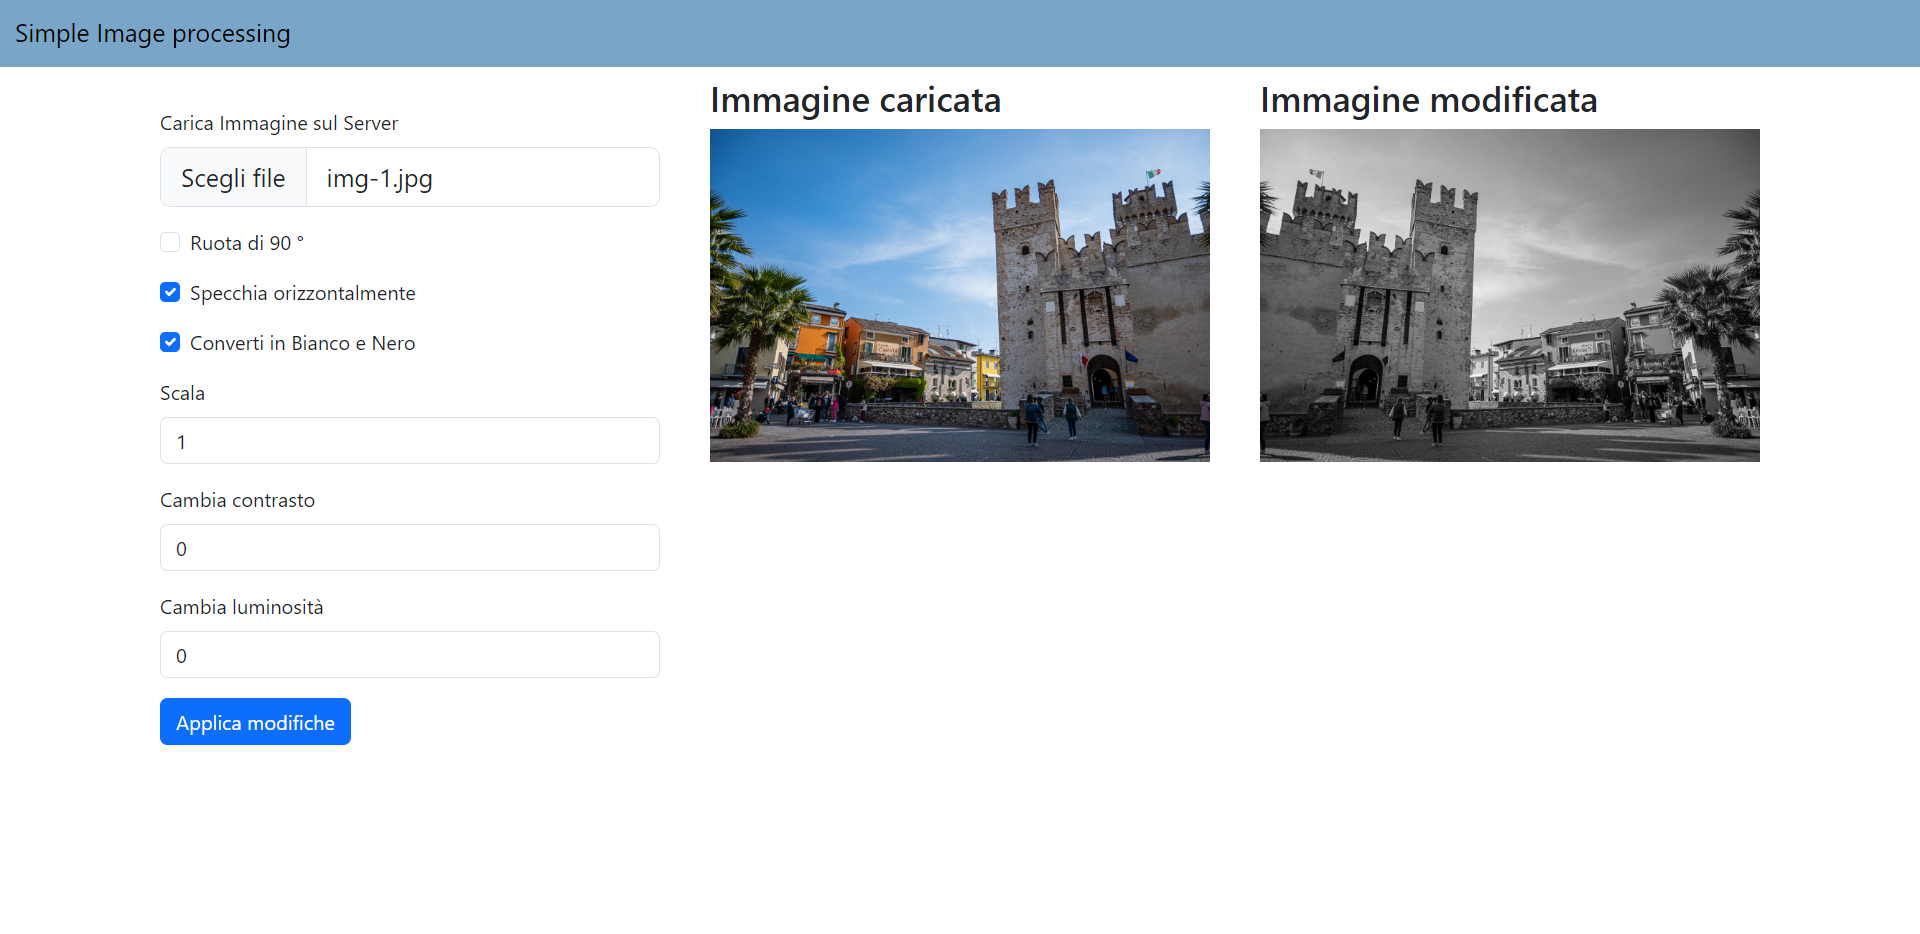
\includegraphics[width=1\columnwidth]{images/client.png}
    \end{center}
    \caption{Pagina html del client}
    \label{fig:client}
\end{figure}
\subsection{Actix-Web}
Lo studio del funzionamento di base del framework Actix-Web ha costituito un punto focale durante la prima fase dell'implementazione.
Tale framework si è dimostrato estremamente flessibile ed adatto per lo sviluppo di un prototipo come quello di questa tesi. Grazie infatti agli \textbf{extractors}, agli\textbf{handlers} e ad altre funzionalità presenti, la gestione di richieste HTTP risulta semplice ed immediata.
Si è deciso di strutturare l'applicazione in diversi file, garantendo così una maggior pulizia e manutenibilità del codice. Il file principale è \textbf{main.rs}.
\begin{lstlisting}[language=rust, label=lst:RustWasi, caption={Porzione del file main.rs}, showstringspaces=false]
#[actix_rt::main]
async fn main() -> std::io::Result<()> {
    HttpServer::new(move || {
        App::new()
            .route("/", web::get().to(server::handlers::index))
            .route("/upload", web::post().to(server::handlers::upload))
            .service(fs::Files::new("/script", "./src/static/"))
            .service(fs::Files::new("/img", "./img/"))
            .app_data(state.clone())
    })
    .bind("127.0.0.1:8080")?
    .run()
    .await
}
\end{lstlisting}
Come si può notare è presente la creazione di un HttpServer e di un istanza di App. Tutti i server actix-web sono costruiti attorno all'istanza di App.
\textbf{è presente lo state!!!!! cosa fare???} Essa permette infatti, di configurare "regole di ruoting" per risorse di vario tipo, di registrare servizi HTTP e anche di contenere stato di livello applicazione. 
\\Nel nostro caso sono state configurate due regole di routing. La prima prende in considerazione richieste eseguite alle home del sito, mentre la seconda gestirà richieste per l'upload e la successiva modifica di file. Si noti che entrambe le regole di routing mappano le richieste a funzioni presenti all'interno del file \textbf{handlers.rs} nel modulo server.
\\Successivamente sono stati registrati due servizi HTTP. Entrambi vengono utilizzati per garantire l'accesso a risorse statiche come script Javascript o immagini elaborate dall'applicazione.
\\Infine, dopo aver stabilito il metodo di dispatching delle richieste ed aver messo a disposizione le risorse necessarie ai clienti si è passati alla scrittura del codice del file "handlers.rs". Tale file, come suggerito dal nome, contiene gli handler delle richieste HTTP, con la conseguente esecuzione di codice WebAssmebly per richieste di modifica di immagini.

\begin{lstlisting}[language=Rust, showstringspaces=false]
    #[derive(MultipartForm)]
    pub struct ImageUpload {
        image: TempFile,
        scala: Text<f32>,
        contrasto: Text<f32>,
        luminosita: Text<i32>,
        ruota: Text<bool>,
        specchia: Text<bool>,
        bw: Text<bool>
    }
    pub async fn index() -> HttpResponse {
        HttpResponse::Ok().content_type("text/html")
            .body(include_str!("../static/index.html"))
    }
    let new_file_name = SystemTime::now().duration_since(SystemTime::UNIX_EPOCH).unwrap();
    let filepath = format!("img/uploaded/{:?}_{}",new_file_name, form.0.file_name.as_str());
    match form.0.image.file.persist(filepath) {
            Ok(_) => {
                
                let editings = Editings{
                    scala : form.0.scala.0,
                    ...
                };
                edit(editings)
            },
            Err(e) => {
                HttpResponse::InternalServerError().finish()
            },
        }
    }
\end{lstlisting}
Dal listato precedente si possono facilmente notare i due endpoint per le richieste alla pagina home e per richieste di upload.
Per quanto riguarda la prima tipologia di richieste si risponderà ai client semplicemente con un file HTML statico.
\\Al contrario la gestione delle richieste di upload è notevolmente più complessa e per questo motivo si è deciso di utilizzare una funzione di supporto \textbf{edit()} che si occuperà dell'istanziazione del modulo WASI e della sua esecuzione.
\\Nel frattempo si noti che la funzione "upload" riceve come parametro un MultipartForm.
Il framework Actix-Web (ed in particolare il crate actix-multipart) facilita molto la gestione di richieste provenienti da form contenenti campi di input di tipo "file".
La struct ImageUpload rifletterà i campi contenuti all'interno del form HTML, garantendo in questo modo accesso immedato ai valori inviati al server.
La funzione quì analizzata rende persistente il file temporaneo ricevuto ed inoltre crea una \emph{struct} di supporto che verrà sfruttata dalla funzione edit(). Tale funzione verrà invocata se e solo se il file è stato reso persistente senza errori.
\subsection{Integrazione modulo Wasm/WASI}
Come già sottolineato, per l'esecuzione di codice WebAssmebly, si è deciso di utilizzare il runtime environment \textbf{Wasmtime}. La sua integrazione all'interno di un'applicazione Rust è resa possibile primariamente grazie ai crate \textbf{wasmtime}, \textbf{wasmtime-wasi} e \textbf{wasi-common}.
\subsubsection{Scambio di dati}
Prima ancora di iniziare l'implementazione è stato necessario trovare un modo per scambiare dati tra il modulo WebAssmebly e l'host. Per lo scopo di questo prototipo è necessario che il modulo WebAssmebly riceva tutte le elaborazioni da effettuare su un'immagine e il nome del file da modificare, ma come introdotto in sezione \ref{subsub:Valori} una funzione WebAssmebly può accettare solamente valori di tipo numerico.
\\Grazie alle API WASI sono possibili diverse soluzioni a questo problema, come ad esempio l'utilizzo della memoria lineare, la scrittura su file, la modifica di variabili d'ambiente o la comunicazione tramite standard input.
Alcuni degli approcci presentati risulterebbero però complicati da implementare e dato che per la nostra applicazione sarebbe sufficiente scambiare una stringa per ottenere tutte le informazioni necessarie si è optato per la comunicazione via \textbf{standard input}.
\\In particolare verranno effettuate le seguenti operazioni:
\begin{itemize}
    \item Serializzazione in formato JSON della struct "Editing" contenente tutte le elaborazioni  e il nome del file da modificare;
    \item Messa a disposizione sullo standard input del modulo Wasm della stringa ottenuta dalla serializzazione;
    \item Lettura della stringa dallo standard input del modulo WASI;
    \item Deserializzazione in una Struct Editing equivalente a quella di partenza;
\end{itemize}
\subsubsection{Condizioni necessarie per l'esecuzione}
Prima di poter eseguire un modulo tramite Wasmtime, sono necessarie diverse operazioni preliminari:

\begin{lstlisting}[language=rust, label=lst:RustWasi, showstringspaces=false]
let serialized_input = serde_json::to_string(&editing);
let stdin = ReadPipe::from(serialized_input);

let engine = Engine::default();

let mut linker: Linker<WasiCtx> = Linker::new(&engine);
wasmtime_wasi::add_to_linker(&mut linker, |s| s); 
let  image_directory = Dir::open_ambient_dir("img", ambient_authority());
\end{lstlisting}
Dopo la serializzazione della struttura dati, la prima operazione necessaria è la creazione dell'Engine Wasmtime. Esso è un contesto globale per la compilazione e l'esecuzione di moduli Wasm, che nel nostro caso adotterà la configurazione di default.
\\Si procederà poi con l'istanziazione di un linker. Il linker sarà colui che istanzierà.


\subsection{Modulo WebAssmebly/WASI}

\newpage
\section{Implementazione in Node.js}

\section{Valutazione delle prestazioni}
\section{Qualità del codice e manutenibilità}
\section{Esperienza di sviluppo}
\section{Scalabilità e concorrenza}
\section{Conclusioni}
\section{Sviluppi futuri}